\chapter{Monte Carlo Generators}
\thispagestyle{empty}


As we have seen in the collisions between high energy protons, hundreds of particles are generally present in the final state.
Given the complexity of the events it is necessary to use Monte Carlo generators, i.e. programs that allow to simulate the realistic result of the collisions assuming a certain model for the processes involved and which are the object of the study.
The use of Monte Carlo generators is necessary because it is impossible to predict \textit{a priori} what happens event-by-event: in fact, as we know, in quantum mechanics we can only calculate the probability of having a certain result.
The simulation of an event is carried out in successive steps \cite{Sjostrand: 2006su, Buckley: 2011ms}, as schematized in Fig. \Ref{general}, thus subdividing the problem into several parts of lower complexity.


\begin{figure}
\centering
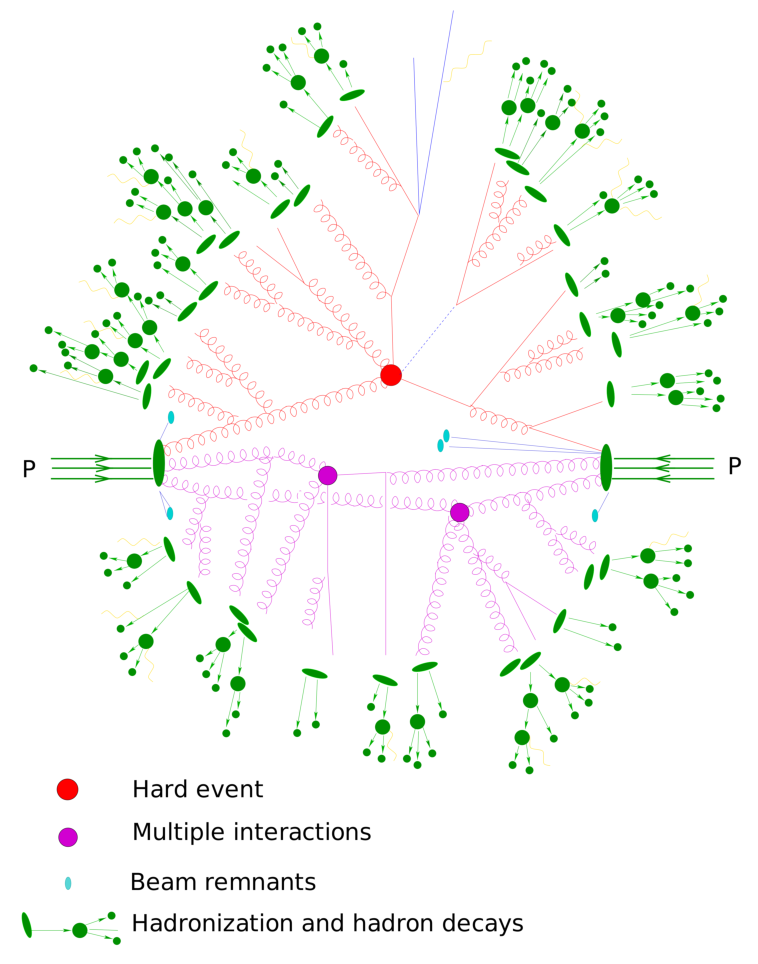
\includegraphics[scale= 1]{../Cap3/Fig_MC/generalMC}
\caption{Schematic representation of an event generated within an event generator. The partons coming from the protons indicative participate in both the hard process and multiple interactions. Subsequently there is an hadronization.}
\label{general}
\end{figure}
The various steps are summarized here:
\begin{itemize}

\item Hard process: the incident protons are made up of partons (quarks and gluons) and the hard process consists of a collision between two partons, coming from different hadrons. The process matrix element can be calculated perturbatively and often only the lowest perturbative order called leading order (LO) is calculated.
\item Parton shower: the incoming or outgoing partons participating in the hard process can emit gluons: in fact, in analogy with the electromagnetic interaction, a particle with an accelerated color charge can radiate for bremsstrahlung.
The gluons in turn can produce quark-antiquark pairs thus generating swarms of partons or parton showers.
The emission of additional partons takes place mainly in a collinear manner with respect to the initial parton and to progressively lesser energies.
In the final state there will be a set of partons, called jet, located in the collinear zone at the initial parton.
This probabilistic process can be simulated as a Markov \cite{Markov1907eot} process and is implemented in the parton shower algorithms we will discuss later.
\item Multiple interactions: the incident protons have been bound to strongly interacting parties. In a single collision, it may therefore happen to have more pairs of partons interacting with each other. In this case it is said that there are multiple interactions in addition to the hard process.
\item Horizing: In the evolution of the event the partons are gradually generated with ever lower relative impulses. For impulse values ​​of the order of 1 \GeV the confinement forces prevail. At these energy scales, perturbation theory fails in the description, so we resort to non-perturbative models
which describe the formation of real hadrons. This process of atomization preserves the jet structure which can therefore be observed experimentally.
\item Decaying of unstable particles: many of the particles produced in the primary process or in the array are unstable and are decayed unless they can interact directly with the detector.

\end{itemize}

The Monte Carlo simulation methods allow these steps to be considered sequentially: the result of each step is the starting point of the next step.
At the end in a single event there are hundreds of particles each of which has a dozen degrees of freedom (mass, flavor, impulse, average life, spin, peak production, etc.), so you can guess the high number of parameters that come into play and must be simulated for each event.
The final aim is to provide a realistic description of what happens in high-energy collisions, in order to compare the Monte Carlo model with the experimental data and see if we are facing unexpected events, which could indicate new physics.
Schematically, the impact section of the final state is given by,
\begin{equation}
 \sigma_{final \: state}=\sigma_{hard \: process} \: \mathcal{P}_{tot, \:hard \: process \rightarrow final \:state} \: \mbox{,}\end{equation}
integrated over the entire phase space and added to all possible final states (for example, the production of two or more jets). This is the measurable quantity associated with the hard process. \\




\section{\textit{Hard process}}

In many processes of interest to LHC high pulses come into play, to produce particles with high mass or very energetic \ textit {jet}. The simulation of these events is the central part of the Monte Carlo generators.
The cross section for a \ textit {scattering} $ ab \ rightarrow n $ process is given \ cite {Buckley: 2011ms} by,

\begin{eqnarray}
 \sigma & = & \sum_{a,b}  \int_{0}^{1} \, dx_{a} dx_b \int f_{a}^{h_1} (x_a , \mu_F) f_{b}^{h_2} (x_b , \mu_F) \: d \hat{\sigma}_{ab \rightarrow n}(\mu_F , \mu_R)  \nonumber \\
& = & \sum_{a,b}  \int_{0}^{1} \, dx_{a} dx_b \int d \Phi_n  f_{a}^{h_1} (x_a , \mu_F) f_{b}^{h_2} (x_b , \mu_F) \nonumber \\
 & \times& \frac{1}{2\hat{s}} 
 | \mathcal{M}_{ab \rightarrow n} 
(\Phi_n , \mu_F , \mu_R)|^2  \: \mbox{,} \end{eqnarray}
where




\begin{itemize}
\item $f_{a}^{h} (x , \mu)$ are the partitioning functions (PDF) that depend on the $x$ fraction of the energy of the parton $a$ (Bjorken variable) with respect to the $h$, and on the $\mu_F $ factorization scale, which we had introduced already in the Eq. XX.
\item $\hat {\sigma}_ {ab\rightarrow n} $ is the partonic cross section of the process $ ab \rightarrow n $.
The total differential cross section is given by the product of the corresponding square matrix element, $ | \mathcal {M}_{ab \rightarrow n} |^2 $, and from the flow of incident plots $ 1 / (2 \hat{s}) = 1 / (2 x_a x_b s) $, where $ \ sqrt{s } $ is the energy of the system's center of mass.
\item The array element $ | \mathcal{M}_{ab \rightarrow n} (\Phi_n, \mu_F, \mu_R) |^2 $ can be written as the sum on all Feynman diagrams,
are the partitioning functions (PDF) that depend on the $ x $ fraction of the energy of the parton $ a $ (Bjorken variable) with respect to the $ h $, and on the $\mu_F $ factorization scale, which we had introduced already in the Eq. XX.

\item  $\hat{\sigma}_{ab \rightarrow n}$ it is the partonic cross section of the process $ab \rightarrow n$. 
The total differential cross section is given by the product of the corresponding square matrix element, $| \mathcal{M}_{ab \rightarrow n} |^2 $,and from the flow of incident parts $1/(2 \hat{s})= 1/(2 x_a x_b s)$, where $\sqrt{s}$ it is the energy of the mass center of the system.
\item Matrix element $| \mathcal{M}_{ab \rightarrow n}  (\Phi_n , \mu_F , \mu_R) |^2 $ it can be written as the sum on all Feynman diagrams,

\begin{equation}
\mathcal{M}_{ab \rightarrow n}= \sum_{i} \mathcal{F}_{ab \rightarrow n}^{(i)} \: \mbox{.} \end{equation}

\item $d\Phi_n$ it is the phase space differential for $ n $ particles in the final state.
\end{itemize}

 The phase space will not be all physical space possible but will contain cuts for two reasons: on the one hand the cuts will reflect the geometry and acceptance of the detector; on the other hand it is almost always necessary a cut on the transverse impulse of the particles produced in the process to avoid divergences in the calculation of the cross section \footnote {You can imagine having a singularity similar to that one has in scattering  classic coulomb.}.
In general, the calculation of the matrix element would require the calculation of all the Feynamn diagrams which in fact grow in a factorial way (Fig.~\ref{fatt}) with the number of particles in the final state.

\begin{figure}[h]
\centering
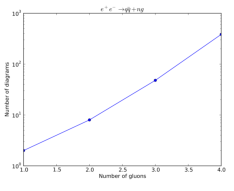
\includegraphics[scale= 2.5]{../Cap3/Fig_MC/fattoriale}
\caption{ \textit{Trends in the number of Feynman diagrams as the number $ n $ of gluons increases in the process $e^+ e^- \rightarrow q \bar{q} + ng$}.}
\label{fatt}
\end{figure}
Most event generators can compute the leading order of the known process matrix element within the Standard Model of the type $2 \rightarrow 1$,  $2 \rightarrow 2$
and also  $2 \rightarrow 3$ \cite{bib:madgraph}.  \\
However, if we stopped at the first perturbative order, we would have only a rough description of the process: in fact, subsequent orders involve important corrections both to the shape of the distributions and to the total cross section. LO is useful for a first study but, where possible, it is important to evaluate next-to-leading-order (NLO) \footnote{For some particularly important processes, for example $ gg \rightarrow H $, the next-next-to-leading-order (NNLO) calculations are even available.}. \\
The cross section calculated at the NLO is composed of three parts: from the LO or part of Born, and from the real and virtual corrections to the emission (Fig. \ref{nlofig}),

\begin{equation}
 \label{xsecNLO}
 d\sigma^{NLO} =  d \tilde{\Phi}_n [\mathcal{B} (  \tilde{\Phi}_n  ) + \alpha_s \mathcal{V}(  \tilde{\Phi}_n  ) ] +  d \tilde{\Phi}_{n+1} \alpha_s \mathcal{R}(\tilde{\Phi}_{n+1}  ) \: \mbox{,}   \end{equation}
 where $\mathcal{B}$, $\mathcal{R}$ and $\mathcal{V}$ they denote the part of Born, the real part and the virtual part respectively. The integral must be made on all the $ n $ or $ n + 1 $ final state particles and on the Bjorken variables related to the incident parts.
Suppose that in the Born approximation the process is of the type $ 2 \rightarrow 2 $. If you want to go to the next order, NLO, you have to keep the chart with an additional part in the final state, $ 2 \rightarrow 3 $ process, and virtual correction with a loop in the $ 2 \rightarrow 2 $ process.
It should be noted that the cross-section for processes of the type $ 2 \rightarrow 3 $ is divergent when the energy of one of the partons tends to zero (divergence  soft) or when two parts are collinear (collinear divergence).


\begin{figure}
\centering
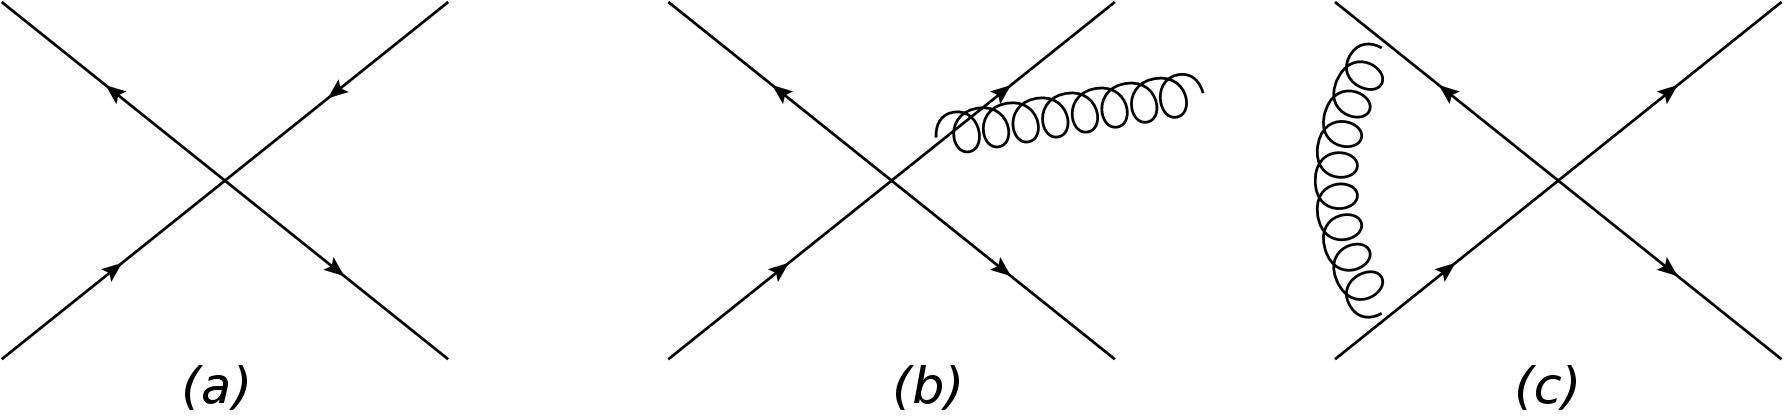
\includegraphics[scale=0.22]{../Cap3/Fig_MC/nlo2}
\caption{ \textit{Examples of Feynman diagrams (a)  Born, (b) real, (c) virtual. }}
\label{nlofig}
\end{figure}

 
\section{\textit{Parton shower}}
In una collisione fra partoni  una carica di colore viene accelerata, quindi sarà presente emissione di \textit{bremsstrahlung}. Quando si studia un processo del tipo $2\rightarrow n$, dove $n$ rappresenta il numero di partoni nello stato finale, l'elemento di matrice al LO (anche detto \textit{tree-level}) avrà delle divergenze nel caso collineare e \textit{soft}. In particolare i processi che soffrono di questo tipo di divergenza sono $q \rightarrow qg$, $\bar{q} \rightarrow \bar{q}g$, $g \rightarrow gg$: i primi sono i processi analoghi a  $e \rightarrow e\gamma$ in QED, mentre il terzo è dovuto al fatto che la QCD non è una teoria abeliana. Il processo  $g \rightarrow q \bar{q}$ invece non ha questo tipo  divergenze.
Le divergenze dell'elemento di matrice \textit{tree-level} possono essere rimosse introducendo nel calcolo le correzioni virtuali, che però saranno all'ordine successivo; questi calcoli dunque risultano particolarmente complessi e sono possibili solo per un  numero limitato  di processi.  Gli algoritmi di \textit{parton shower}  \cite{Sjostrand:2006su} offrono un modo alternativo e abbastanza semplice per eliminare le divergenze collineari e \textit{soft} attraverso:
\begin{itemize}
\item una struttura iterativa che combina in un unico stato finale multi-partonico i tre stati che soffrono delle divergenze,
\item l'introduzione del fattore di forma di Sudakov.
\end{itemize}
I partoni entranti o uscenti, che sono lontani (temporalmente) dall'\textit{hard process}, sono detti \textit{on-shell} perchè il modulo del loro quadrimpulso è uguale alla massa a riposo. Tuttavia più ci si avvicina  all'interazione, a causa del principio di indeterminazione ($\Delta E \Delta t \sim \hbar$),  i partoni possono essere in uno stato detto  \textit{off-shell}, cioè il modulo del loro quadrimpulso non corrisponde alla massa a riposo. Per questo motivo sono in grado di emettere altri partoni e in particolare quanto più sono vicini allo scattering quanto maggiore può essere l’energia dei partoni emessi. Se l’emissione avviene prima dello scattering si parla di radiazione di stato iniziale (ISR), mentre dopo l’interazione di parla di radiazione di stato finale (FSR). \\
Ogni partone è caratterizzato da una scala di ``virtualità'' $Q^2$ che corrisponde in modo approssimato a una scala di  ordine temporale dello sciame. E' importante sottolineare che sono disponibili differenti definizioni per $Q^2$; tuttavia indipendentemente dalla convenzione scelta,  la scala $Q^2$ aumenta  avvicinandosi all'\textit{hard process}, quindi nell'ISR, e diminuisce allontanandosi, nell'FSR. Se prendiamo come esempio la FSR, l’evoluzione inizia ad una scala $Q^2_{max}$ che è legata all’hard process e termina quando si raggiunge una scala limite, $Q_0$, che sarà dell'ordine di 1 GeV.\\
La scelta più comune utilizzata è porre $Q^2=p^2=E^2- |\vec{p}\,|^2$. Con questa convenzione in un processo   di tipo $a \rightarrow bc$, nel caso di FSR, $Q^2 >0$, ovvero di tipo \textit{time-like}, e diminuirà fino a che si raggiunge la scala limite $Q_0$. 
Le cose sono più complicate nel caso ISR: in questo caso $a$ e $b$, supposti qui \textit{off-shell}, hanno  $p^2$ di tipo \textit{space-like}, quindi si ridefinisce $Q_i^2=-m_i^2$ in modo da garantire l'ordine crescente di $Q^2$, i.e. $Q_b ^2 > Q_a ^2$. 
Di contro $c$ non parteciperà all'\textit{hard process} e  avrà $p^2>0$ e quindi il suo sciame evolverà come quello del FSR.
\paragraph{Radiazione di stato finale}


Nell'approccio col \textit{parton shower}  lo stato di radiazione finale è modellizzato attraverso una serie di processi divisionali  del tipo $a \rightarrow bc$.   
Ciò è evidente dal processo   $q \bar{q}g$, Fig. \ref{nlofig} (b), dove le correzioni reali dell'elemento di matrice al primo ordine corrispondono all'emissione di un gluone. L'evoluzione dello sciame è descritta da due parametri: la frazione di energia portata da uno dei due partoni uscenti, $z=E_b/E_a$, e la variabile di ordine $t$. Come abbiamo detto una  possibile scelta per $t$ è la virtualità $Q_a^2$ del partone incidente.
Nel limite collineare la probabilità di divisione $d \mathcal{P}_{a \rightarrow bc}$, espressa in termini di $z$ e $t=\ln(Q^2/\Lambda^2)$ è data da:
\begin{equation}
 d \mathcal{P}_{a \rightarrow bc}= \sum_{bc} \frac{\alpha_{abc}}{2 \pi}\: {P}_{a \rightarrow bc} \:dt dz  \: \mbox{,} \label{prob}  \end{equation}
dove $dt=\frac{d Q^2}{Q^2}$, $\alpha_{abc}$ è la costante di accoppiamento che regola la il processo di divisione e ${P}_{a \rightarrow bc}$ è detto \textit{kernel splitting}; queste sono funzioni  universali e valgono nel limite collineare:

\begin{eqnarray}
P_{q \rightarrow qg    }&=& \frac{4}{3} \frac{1+z^2}{1-z} \mbox{,} \nonumber \\ 
 P_{g \rightarrow gg }&=& 3 \frac{(1-z(1-z))^2}{z(1-z)}    \mbox{,} \\ 
P_{g \rightarrow q\bar{q} }&=& \frac{n_f}{2} (z^2+ (1-z)^2)   \mbox{,} \nonumber \end{eqnarray}
dove $n_f$ è il numero di sapori dei \textit{quark}.
Tuttavia la probabilità così valutata  è superiore all'unità perché soffre  delle stesse divergenze dell'elemento di matrice al LO. Infatti l'espressione \ref{prob} è valutata in approssimazione collineare. In particolare si hanno due tipi di divergenze: collineari, dovute alla dipendenza di tipo $1/Q^2$, e \textit{soft} che corrisponde al limite $z=1$.\\
Per ovviare a ciò, nell'approccio del \textit{parton shower},  come prima cosa si valuta la probabilità di divisione fra $t$ e $t +dt$; questa si ottiene integrando l'Eq \ref{prob} su tutti i possibili  $z$ compresi nell'intervallo $[z_{min}(t), \: z_{max}(t)]$:
\begin{equation}
 d \mathcal{P}_{a \rightarrow bc}= \left( \sum_{bc} \int_{z_{min}(t^{'})}^{{z_{max}(t^{'})}}  \frac{\alpha_{abc}}{2 \pi}\: {P}_{a \rightarrow bc} \:dt dz \right) dt  \: \mbox{.}   \end{equation}
Come in altre situazioni fisiche\footnote{Per esempio il decadimento radioattivo.} e non solo, la probabilità che accada qualcosa a $t$ è data dalla probabilità che ciò avvenga fra  $t$ e $t +dt$, moltiplicata per la probabilità che ciò non sia già avvenuto fra l'istante iniziale $t_0$ e $t$.
In questo caso allora la probabilità di avere una divisione a $t$ è:
\begin{equation}
 d \mathcal{P}_{a}^{\mbox{\footnotesize{FSR}}}(t)=   d \mathcal{P}_{a} \cdot \mbox{exp} \left(   -\sum_{bc} \int_{t_0}^t dt^{'}  \int_{z_{min}(t^{'})}^{{z_{max}(t^{'})}} \frac{\alpha_{abc}}{2 \pi} P_{a \rightarrow bc}(z) dz \right) \mbox{,}\end{equation}
dove $t_{0}$ è la scala di partenza dello sciame. Il termine esponenziale è detto fattore di forma di Sudakov e rappresenta, come intuibile, la probabilità di non divisione.  Se lo si vuole interpretare in termini di diagrammi di Feynman questo rappresenta le correzioni virtuali dell'elemento di matrice LO.\\
Tutto questo procedimento può essere combinato insieme  per avere più emissioni  a differenti passi successivi: si avrà così uno sciame di partoni che sarà ordinato in $Q$ decrescente. Infine è importante sottolineare che la descrizione fornita dal \textit{parton shower} è corretta nel caso si abbiano \textit{jet} collineari e fallisce in configurazioni in cui sono presenti partoni ben separati.
   

\paragraph{Radiazione di stato iniziale}
L'evoluzione della radiazione di stato iniziale è molto più complicata rispetto a quella di stato finale. Infatti \textit{quark} e gluoni sono continuamente emessi e riassorbiti all'interno dei protoni incidenti. Ciò significa che quando avviene l'\textit{hard scattering} la radiazione di stato iniziale è già presente.
Si potrebbe semplicemente pensare di simulare ISR partendo dai partoni \textit{on-shell} prima dell'interazione e facendoli evolvere a scale $Q^2$  sempre più elevate fino a raggiungere  un \textit{hard process}. Questo approccio però è molto inefficiente perché risulta particolarmente raro simulare il processo di interesse dato che  avrebbe la stessa probabilità che ha in natura. Si utilizza allora nei generatori di eventi un approccio differente: come prima cosa viene prodotto l'\textit{hard process} e successivamente si prova a ricostruire all'indietro cosa può essere avvenuto. Questo procedimento prende il nome di ``evoluzione all'indietro'', Fig. \ref{isr} .
Consideriamo, come nel caso FSR, il processo di tipo $a \rightarrow bc$ e valutiamo in questo caso la probabilità che un partone $b$ possa essere stato prodotto dal partone $a$. E' necessario introdurre la funzione di densità partonica; questa  evolve in accordo con l'equazione di DGLAP \cite{Altarelli:1977zs}, 


\begin{figure}
\centering
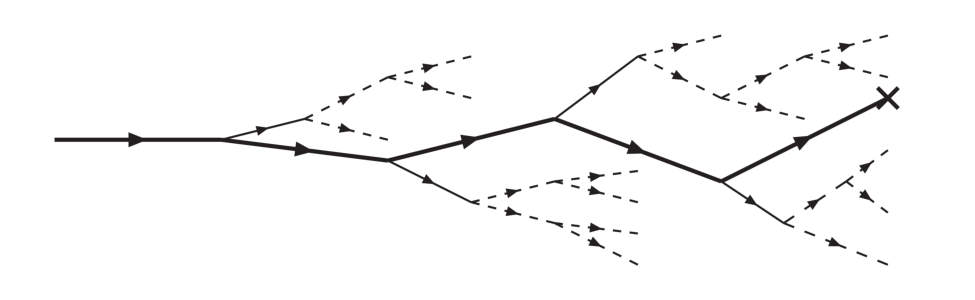
\includegraphics[scale= 0.8]{../Cap3/Fig_MC/isr}
\caption{ \textit{Evoluzione dello stato iniziale. La linea in grassetto corrisponde al partone che subirà l'hard process (rappresentato da una croce). Le linee sottili rappresentano i partoni che non possono ricombinarsi, mentre quelle tratteggiate sono fluttuazioni che possono o non possono ricombinarsi.   }}
\label{isr}
\end{figure}

\begin{equation}
  \frac{d f_b(x, \:t)}{dt}= \sum_{ac} \int_x ^1 \frac{d x^{'}}{x^{'}} \: f_a(x^{'},t) \:\frac{\alpha_{abc}}{2\pi} \:P_{a \rightarrow bc} \:(\frac{x}{x^{'}}) \mbox{,}\end{equation}
dove $f_{a,b}(x, \:t)$ sono le PDF del partone $a$, $b$, che ha ha frazione $x$ dell'impulso del protone incidente e scala $t=\mbox{ln}(Q^2/ \Lambda^2) $, mentre $P_{a \rightarrow bc}$ è  la funzione di \textit{kernel splitting}.\\
Nell'evoluzione all'indietro la probabilità che il partone $b$ sia stato generato da $a$  nell'intervallo di scala fra $t$ e $t-dt$ è data da:
\begin{equation}
d\mathcal{P}_{b}(t)=\frac{d f_b(x, \:t) }{ f_b(x, \:t)}= |dt| \sum_{ac}  \int  \frac{d x^{'}}{x^{'}} \frac{d f_a(x^{'}, \:t) }{ f_b(x, \:t)} \frac{\alpha_{abc}}{2\pi}          \:P_{a \rightarrow bc} \:(\frac{x}{x^{'}})      \mbox{,}\end{equation}
mentre la probabilità di non divisione fra la scala $t_{max}$ e $t<t_{max}$:
\begin{equation}
S_b (x,t,t_{max})=   \mbox{exp} \left( - \int_t ^{t_{max}} dt^{'} \sum_{ac}  \int  \frac{d x^{'}}{x^{'}} \frac{d f_a(x^{'}, \:t^{'}) }{ f_b(x, \:t^{'})} \frac{\alpha_{abc}}{2\pi}          \:P_{a \rightarrow bc} \:(\frac{x}{x^{'}}) \right)     \mbox{,}\end{equation} 
Infine allora la probabilità di ricombinare $b$  in $a$ è data nell'intervallo compreso fra $t$ e $(t-dt)$ da:

\begin{eqnarray}
d \mathcal{P}_{b}^{\mbox{\footnotesize{ISR}}}(t) &=& - \frac{d S_b (x,t,t_{max})}{dt} dt \nonumber \\
&=&  \sum_{ac}  \int  \frac{d x^{'}}{x^{'}} \frac{d f_a(x^{'}, \:t) }{ f_b(x, \:t)} \frac{\alpha_{abc}}{2\pi}          \:P_{a \rightarrow bc} \:(\frac{x}{x^{'}})  \cdot S_b (x,t,t_{max}) dt \end{eqnarray}
In questo caso il fattore di forma si Sudakov è differente rispetto a quello del FSR dato che contiene le PDF.
Questo fa sì che i risultati del \textit{parton shower} non dipendono solo dall’algoritmo ma anche dalle PDF usate.

\paragraph{Risommazione} Quando si calcola un'osservabile della QCD in modo perturbativo, l'espansione in termini in potenze di $\alpha_S$ contiene termini del tipo $\alpha_S^n L^k$ ($k<2n$), dove $L=\ln (q_{cut}/s)$, essendo $q_{cut}$ il taglio sull'emissioni risolvibili. Quando si considerano ``piccoli'' valori di $q_{cut}$ il logaritmo dell'espansione perturbativa diventa grande e può  far divergere la serie perturbativa. 
Il termine di ordine $n$ dell'espansione perturbativa è il più significativo solo se i termini successivi della serie sono trascurabili; tuttavia ciò non è garantito nel caso in cui siano presenti elevati valori di $L$. E' dunque necessario cosiderare i termini che hanno un elevato valore del logaritmo. Lo studio di questi termini è detto risommazione e viene effettuato mettendo insieme i termini nella serie perturbativa in base al loro grado di divergenza: $\alpha_S^n L^{2n}$ sono i termini \textit{leading log}, LL; $\alpha_S^n L^{2n-1}$ sono i termini \textit{next-to-leading log}, NLL, e così via. Alla fine viene effettuata la loro somma a tutti gli ordini di $\alpha_S$. Per  molti processi sono disponibili i calcoli al NLL.
Il \textit{parton shower} riproduce gli effetti della risommazione approssimativamente al NLL.

\paragraph{Combinazione fra ME e PS}
I due differenti approcci del calcolo dell'elemento di matrice e del \textit{parton shower} hanno dei vantaggi e degli svantaggi. Per quanto riguarda il ME si ha:
\begin{itemize}
\item i calcoli dell'elemento di matrice al LO possono essere effettuati esattamente fino a casi in cui sono presente molti \textit{jet} (dell'ordine di sei) nello stato finale.
\item si ha una buona descrizione di partoni separati
\item i calcoli perturbativi sono esatti 
\item tuttavia, la sezione d'urto diverge  nel caso collineare e \textit{soft}, quindi non è possibile una descrizione esaustiva della struttura interna del \textit{jet}.
\end{itemize}
D'altro lato il PS:
\begin{itemize}
\item è un approccio universale che produce una configurazione realistica dei partoni
\item le divergenze, nel limite collineare, sono trattate con l'introduzione del fattore di forma di Sudakov. Dunque si ha un'appropriata descrizione dell'evoluzione del \textit{jet} 
\item tuttavia il metodo fallisce quando si descrivono partoni separati, dato che l'approssimazione collineare in tal caso non può essere valida.
\end{itemize}
Chiaramente i due metodi sono complementari  ed una loro combinazione (o \textit{merge}) è auspicabile. Esistono differenti approcci che combinano il ME con il PS. La difficoltà principale è che non è facile coprire l'intero spazio delle fasi senza sovrapposizioni e buchi: si vuole descrivere  un processo in cui sono presenti $n$ partoni ben separati nello stato finale,  utilizzando sia l'elemento di matrice al LO ma  volendo anche includere la risommazione dei grandi logaritmi (LL, NLL) che è tipica del PS. Una descrizione schematica della combinazione per quattro \textit{jet}  è riportata in Fig \ref{merge} \cite{bib:lenzi}.
Sull'asse orizzontale sono riportati gli ordini di accoppiamento in $\alpha_S$, mentre su quello verticale la potenza del logaritmo.
Il PS descrive il LL ($m=2n$) e il NLL ($m=2n-1$) ovvero le sfere in verde (p.e. nel caso di $n=2$, $m=$4, 3 le due sfere colorate in verde e segnate come ``4'').
Le sfere che  descrivono l'evento con 4 \textit{jet}, combinando il ME con il PS, sono tutte le verdi, quella azzurra, e le tre rosse segnate con il  ``4''.
La difficoltà sorge perché il ME descrive esattamente tutte le sfere segnate con il ``4'': quindi se semplicemente  sommassimo i due approcci avremmo doppi conteggi delle sfere verdi denominate ``4''.    
\begin{figure}
\centering
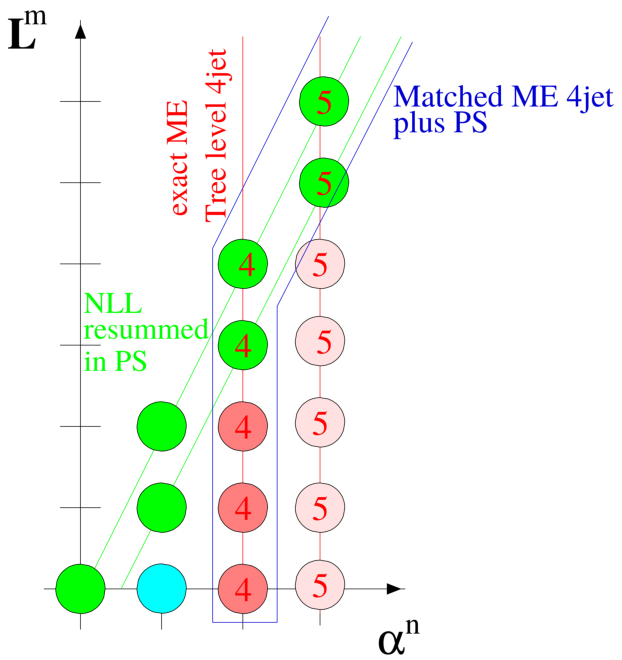
\includegraphics[scale= 0.7]{../Cap3/Fig_MC/merge}
\caption{ \textit{Rappresentazione schematica della combinazione fra ME e PS.   }}
\label{merge}
\end{figure}
I  principali approcci che combinano ME e PS sono:
\begin{itemize}
\item Ripesamento del \textit{parton shower}: l'idea di base  è partire  dal processo all'ordine più basso e successivamente ripesare l'emissione del PS come se fosse stata prodotta dal ME. Questo approccio non cambia la sezione d'urto, che rimane all'ordine più basso, ma migliora il popolamento dello spazio delle fasi \cite{ripesamento, ripesamento2}.  
\item Prescrizione CKKW: lo spazio delle fasi viene suddiviso in due zone utilizzando $k_{\perp}$ che è una misura del taglio $Q_0 ^2$: la regione in cui è prodotto il \textit{jet} è riempita con il ME, quella di evoluzione con il PS \cite{ckkw, ckkw2}. 
\item La prescrizione  MLM, che è pure molto diffusa, si basa sullo stesso principio, ma è  implementata in un modo diverso. 
\end{itemize}


\section{Interazioni multiple}
I protoni incidenti che partecipano all'interazione sono composti da un gran numero di partoni (\textit{quark} e gluoni) che possono interagire in modo indipendente gli uni con gli altri in aggiunta all'\textit{hard-process}.
La sezione d'urto totale per il processo di QDC $2\rightarrow2$ è dominata dal processo $t$, quindi la sezione d'urto diverge come $d p_{\perp}^2/p_{\perp}^4$ per $p_{\perp} \rightarrow 0$  \cite{Sjostrand:2006su}.
Dunque quando si simula un evento reale, in aggiunta all'evento \textit{hard}, caratterizzato dall'avere grandi impulsi trasversi trasferiti, si deve tener conto anche delle collisioni aggiuntive a piccolo  $p_{\perp}$. Se queste avvengono in modo indipendente allora ci si aspetta un distribuzione di Poisson, $P_n= \langle n \rangle^n \mbox{exp}(-\langle n \rangle)/n! $. Tuttavia la conservazione dell'energia e dell'impulso fa si che le interazioni non siano effettivamente indipendenti  sopprimendo così la possibilità, per $p_{\perp} \rightarrow 0$, di avere un elevato numero di interazioni. 
Va inoltre osservato che per eliminare la divergenza è necessario introdurre un valore di \textit{cut-off} dell’impulso trasverso, al di sotto del quale non si generano  collisioni.



\section{Adronizzazione}
Il processo di adronizzazione, in questo contesto, è un particolare modello, utilizzato nei generatori di eventi, che descrive il passaggio dallo stato partonico finale allo stato adronico finale, che  è un'osservabile sperimentale.  E' importante sottolineare che questa transizione è trattata in modo fenomenologico e  non mediante un approccio rigoroso.  Le due più importanti classi per l'adronizzazione sono il modello a stringhe e quello a \textit{cluster}. La differenza è che il primo trasforma i sistemi partonici direttamente in adroni, mentre il secondo compie un passo intermedio dove raggruppa gli oggetti ad una scala dell'ordine di $\sim 1$ GeV.

\paragraph*{Modello a stringhe}
Il più completo ed esauriente ``modello a stringhe'' è quello di Lund: sappiamo dalla  QCD  che fra partoni è presente una forza di confinamento lineare che aumenta con la distanza. Consideriamo, come esempio, lo stato finale in cui sono presenti due \textit{quark}, $ q \bar{q}$. Come i partoni si allontanano il tubo di flusso di colore viene ``stirato'' fra $q$ e $\bar{q}$, Fig. \ref{tubo} (a). Le dimensioni trasverse del tubo sono quelle tipiche adroniche, quindi di circa 1 fm.
Se il tubo è assunto essere uniforme, il potenziale cresce linearmente, $V(r)=\kappa r$, con $\kappa \approx$ 1 GeV/fm, costante della stringa.
\begin{figure}
\centering
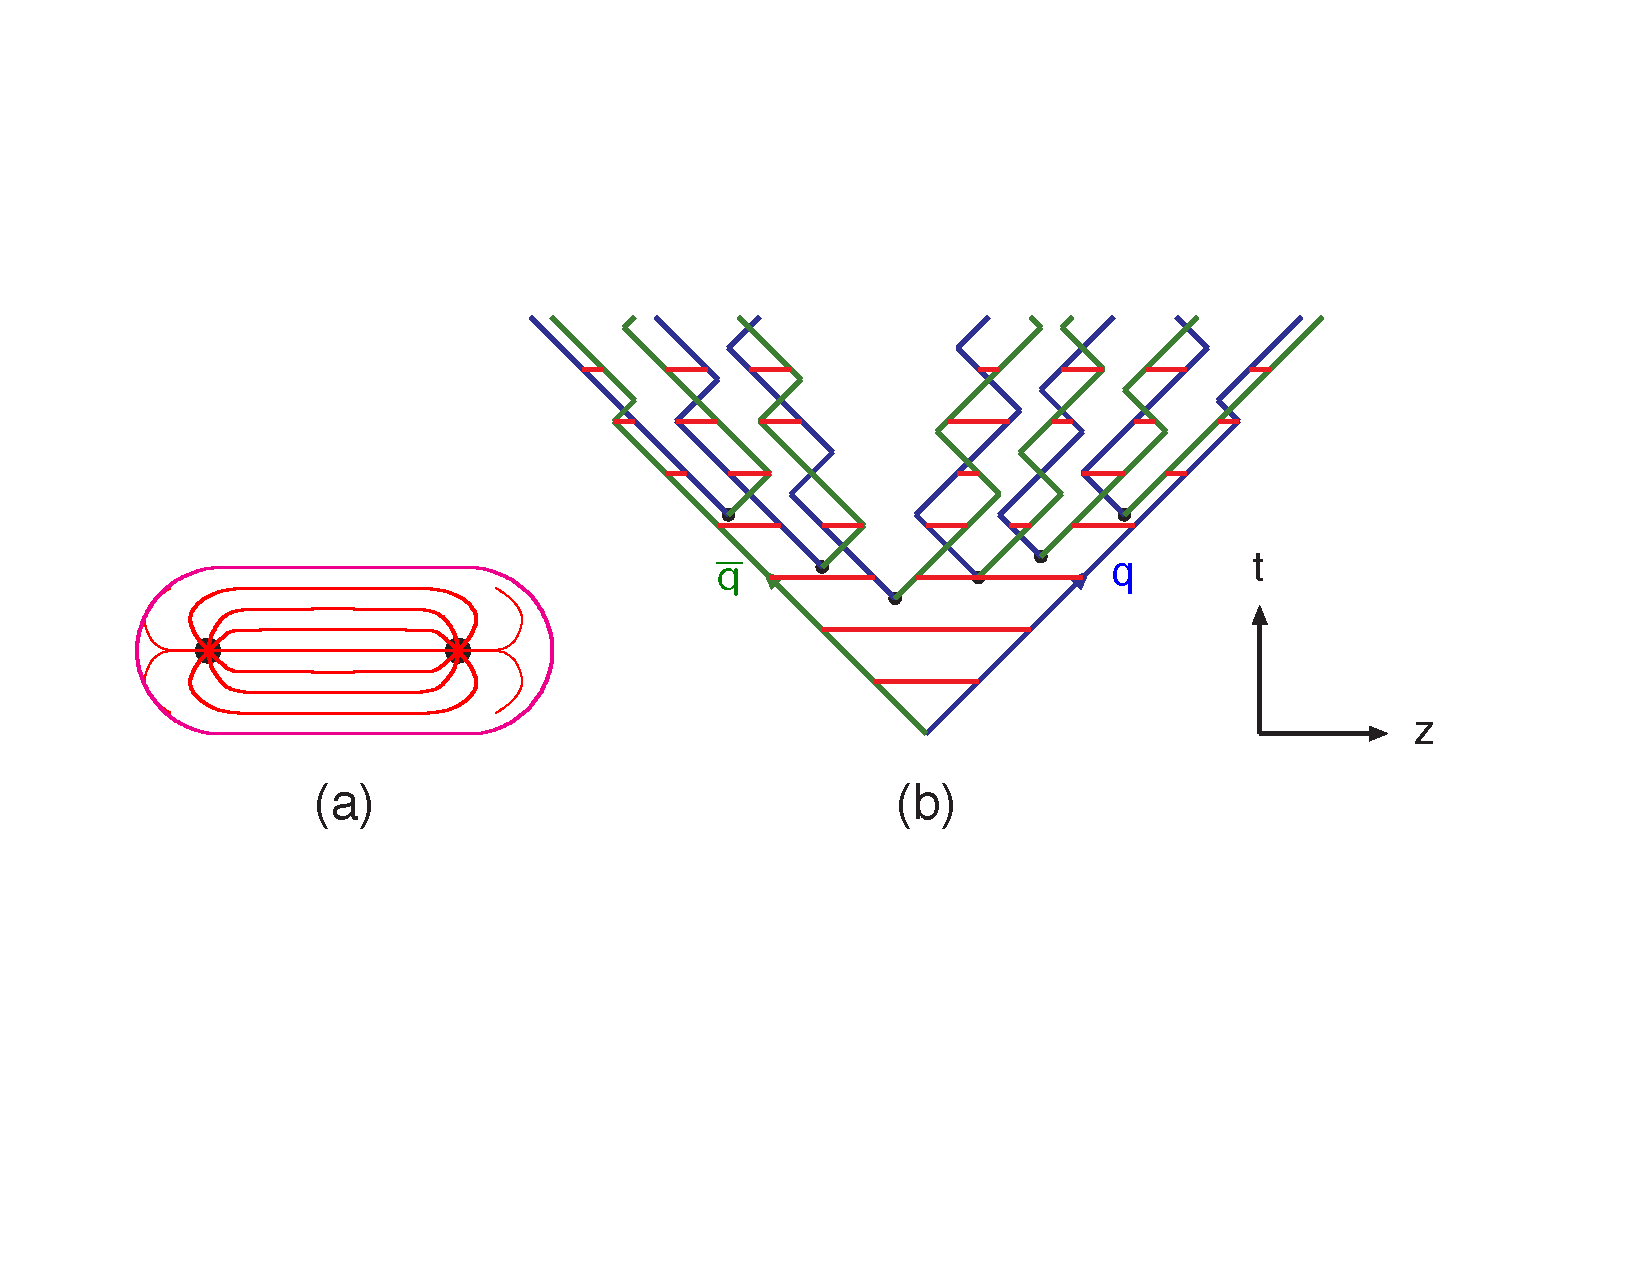
\includegraphics[scale= 0.5]{../Cap3/Fig_MC/stringone}
\caption{(a) \textit{Il tubo di flusso presente fra un quark e un antiquark che si allontanano.} (b) \textit{Moto e rottura di una stringa del sistema.}}
\label{tubo}
\end{figure}
A corte distanze sarebbe necessario introdurre un termine di Coulomb aggiuntivo, $\sim \frac{\alpha_s}{r}$, tuttavia nel modello di Lund si assume questo termine trascurabile.
Come il \textit{quark} e l'\textit{antiquark} si allontanano del vertice di creazione, l'energia potenziale accumulata nella stringa aumenta fino a che non si rompe dando origine ad una coppia $q' \bar{q}'$. Così il sistema si divide in due nuovi singoletti di colore $q \bar{q} '$ e $q' \bar{q}$. Questi due sistemi si allontaneranno a loro volta ripetendo  il processo appena descritto. L'evoluzione del sistema nello spazio-tempo è rappresentata in \ref{tubo} (b).
Alla fine del processo si avrà una seri di coppie $q_i \bar{q_i}$, ognuna delle quali formerà un adrone.
Per ora  è stato considerato solamente il caso $q \bar{q}$. Tuttavia se più partoni provengono dall'interazione il modello a stringhe diventa più complicato. Per un evento in cui è presente un gluone  aggiuntivo, $q \bar{q} g$, la stringa è tesa fra $q$ e $g$ e fra $g$ e $\bar{q}$, Fig. \ref{tubo3}. 
\begin{figure}
\centering%
{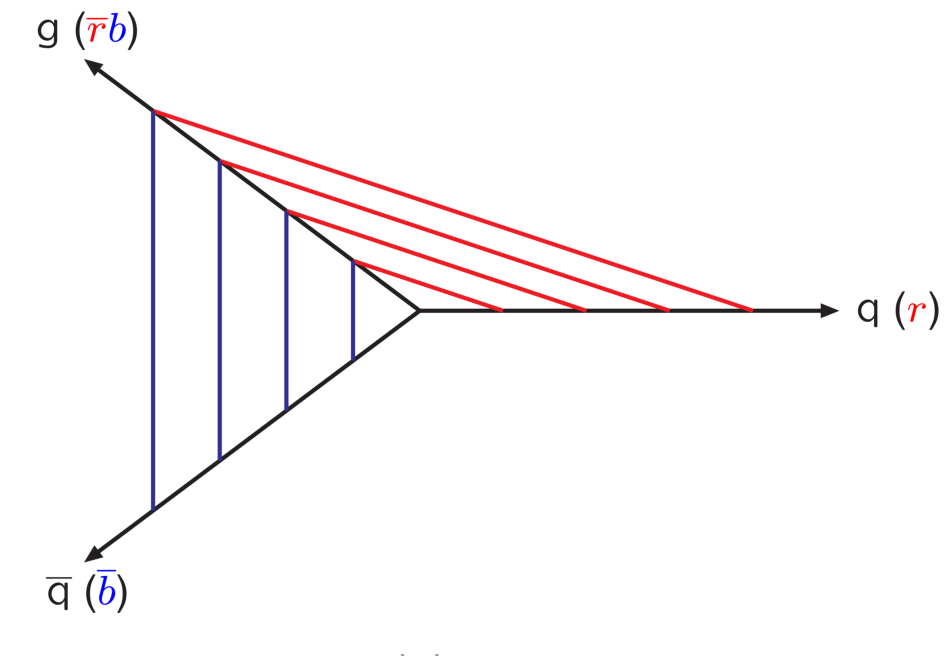
\includegraphics[scale= 0.5]{../Cap3/Fig_MC/stringtwo22}}
\caption{ \textit{Moto della stringa nel caso $q \bar{q}g$.}}
\label{tubo3}
\end{figure}

\begin{figure}
\centering%
\subfigure[]%
{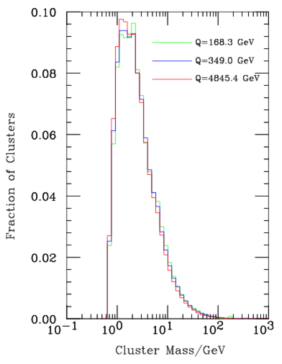
\includegraphics[scale= 1.5]{../Cap3/Fig_MC/split2}}
\subfigure[]%
{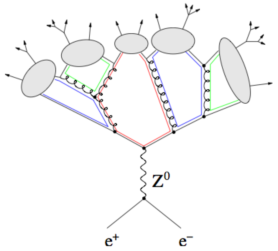
\includegraphics[scale= 1.4]{../Cap3/Fig_MC/split}}
\caption{(a)  \textit{Struttura del parton shower nel modello cluster.} (b) \textit{Distribuzione di massa invariante per singoletti.}}
\label{tubo2}
\end{figure}


\paragraph*{Modello \textit{cluster}}  Questo modello di adronizzazione è basato sulla proprietà di preconfinamento del \textit{parton shower}: la massa invariante di una singola coppia di partoni con colore opposto è la stessa  a qualsiasi scala $Q^2$. Questa distribuzione ha il suo massimo ad una massa  che è circa il \textit{cutoff} del \textit{parton shower} e  decresce  rapidamente verso lo zero, Fig \ref{tubo2} (a).\\
Nel modello, i gluoni del \textit{parton shower}, sono rappresentati da coppie di linee colore-anticolore connesse al vertice. Ogni linea di colore, in prossimità del  \textit{cutoff}, è collegata con un'altra linea di anticolore presente alla  stessa scala. A questo punto le linee contigue di colore/anticolore sono interpretate, nel limite non perturbativo, come  coppie \textit{quark-antiquark} che danno origine a  mesoni, i quali sono gli oggetti osservabili nello stato finale.
Questo  meccanismo è rappresentato in \ref{tubo2} (b).

\section{Decadimenti adronici e radiazione elettromagnetica.}
Nella fase di adronizzazione possono essere prodotti  adroni instabili che decadono  in altre particelle. Dunque lo stato finale dell'evento è il risultato della convuluzione fra l'adronizzazione e il decadimento. Le informazione necessari per la simulazione delle particelle instabili del decadimento sono generalmente presa dal ``Particle Data Book'' (PDG) \cite{bib:pdg} che fornisce le proprietà (p.e. vita media) di un gran numero di particelle.
In generale, in un generatore di eventi, è necessario scegliere quali adroni includere nella simulazione e successivamente scegliere i possibili canali di decadimento. Oltre ai decadimenti adronici, risulta necessario simulare anche l'emissione di radiazione elettromagnetica. L'approccio più comune adottato è quello di utilizzare algoritmi analoghi a quelli utilizzati per simulare l'emissione di QCD nel \textit{parton shower}.

\section{Ricostruzione dei \textit{jet}}
\label{rico_jet}
Successivamente all'adronizzazione e al decadimento delle particelle instabili è possibile stimare il quadrimpulso dei partoni generati nell'\textit{hard process}  dalla direzione e dall'energia dei \textit{jet} che vengono ricostruiti a partire dalle particelle nello stato finale \cite{bib:run2jet, mass:in:dijet}.
La ricostruzione dei \textit{jet} è affidata ad appositi algoritmi; questi introducono la variabile  distanza, $d_{ij}$, fra due oggetti (particelle o pseudo-\textit{jet}) definita da,
\begin{equation}
d_{ij}=\mbox{min}( k_{ti}^{2p}, k_{tj}^{2p})  \frac{\Delta_{ij}^2}{R^2} \mbox{,}\end{equation}
dove $\Delta_{ij}^2=(y_i - y_j)^2+ (\phi_i - \phi_j)^2$ mentre $k_{ti}$, $y_i$ e $\phi_i$ sono rispettivamente l'impulso trasverso, la rapidità e l'angolo azimutale di $i$. Invece $R$ è il parametro radiale. Si introduce inoltre la distanza fra un oggetto $i$ e il fascio (\textit{beem}), $d_{iB}=k_{ti}^{2p}$ \\

Gli algoritmi procedono calcolando la distanza $d_{ij}$ e fra tutte le coppie di particelle $i$,  $j$ identificando  la minore. Per le due particelle con distanza più piccola si sommano i quadripulsi. Si valuta inoltre   $d_{iB}$ per ogni $i$ e se è minore della distanza  $d_{ij}$ con tutte le altre particelle $j$,  $i$ è considerato un \textit{jet} e viene rimosso   dalla lista degli oggetti presenti nell'evento. 
Infine le distanze vengono ricalcolate e tutta questa procedura è ripetuta finché non si trovano più oggetti da sommare.
Il valore di $p=-1$ definisce l'algoritmo   \textit{anti-}$k_t$ \cite{Cacciari:2008gp}, che è quello utilizzato, mentre   il parametro libero $R$ è stato posto  uguale a 0.5.

\section{Validazione Monte Carlo}
Come già accennato, le simulazioni Monte Carlo sono utilizzate in fisica delle particelle per confrontare le predizioni teoriche con i dati. Inoltre dall'analisi dei dati dei processi previsti nel Modello Standard è possibile ricavare i parametri liberi della teoria che possono essere così inseriti in \textit{input} all'interno dei  generatori di eventi. 
Tuttavia quando si simula un evento con un generatore è importante distinguere la ``verità Monte Carlo'' dalle ``osservabili fisiche''. 
Infatti può essere utile dividere il processo di interesse in vari sotto-processi intermedi come, per esempio, lo stato iniziale   o la produzione di una risonanza. 
Questi oggetti intermedi non sono osservabili fisiche ed in pratica non è possibile effettuare misure dirette o indirette. Contrariamente, nel mondo simulato, è possibile accedere a questi oggetti, e di conseguenza anche alle variabili che li caratterizzano (p.e. $p_{\perp}$, $\eta$, $\dots$).
In aggiunta, nella modellizzazione, è possibile (e conveniente) produrre, in modo distinto,  eventi di solo segnale (S) e di solo fondo\footnote{Per fondo si intende tutti gli eventi che producono  stati finali analoghi a quelli di segnale.} (B).\\
In questo contesto, la validazione dei generatori Monte Carlo consiste nel confrontare i risultati con quelli di altri generatori, con le predizioni dei calcoli analitici e dove possibile con i dati. È superfluo aggiungere che la validazione del generatore Monte Carlo permette molto spesso anche di trovare  errori (\textit{bug}) nel codice di analisi. 
\paragraph*{Rivet} 
Uno dei principali strumenti per la validazione dei Monte Carlo è Rivet (\textit{Robust Independed Validation of Experiment and Theory}) \cite{Buckley:2010ar}; questo programma offre un insieme di analisi \textit{standard} con le quali è possibile verificare l'accuratezza di un dato generatore. In aggiunta l'utilizzatore può scrivere una sua propria analisi utilizzando tutti i componenti di Rivet e questa analisi diventa poi un \textit{plugin} che può essere aggiunto alle librerie in C++ del programma..
Rivet permette di visualizzare i risultati dell'analisi in  istogrammi fornendo in aggiunta, nella parte inferiore del grafico, anche il rapporto fra il numero di eventi presenti nei differenti campioni utilizzati (se più di uno).


\section{Generatori principali}
Per la fisica delle alte energie sono disponibili differenti generatori Monte Carlo.  Ognuno di questi ha metodi differenti per combinare il  ME con il  PS.
Qui ci concentreremo in particolare su  \aMC  interfacciato con  P{\footnotesize YTHIA},   P{\footnotesize OWHEG} -anch'esso interfacciato con   P{\footnotesize YTHIA}- e S{\footnotesize HERPA}. 


\paragraph{Madgraph\_aM{\footnotesize C@NLO}}
L'approccio di \aMC \cite{bib:madgraph} è molto ambizioso, infatti lo scopo di questo  generatore è  calcolare la sezione d'urto al NLO includendo nel calcolo sia  i contributi reali che virtuali. L'\textit{hard process} è prodotto col metodo del ME mentre l'emissioni \textit{soft} e collineare col PS.
Il primo passo è calcolare le correzioni al NLO del ME per un processo a $n$ partoni, includendo   $n+1$ partoni provenienti dalle correzioni reali ed  $n$ provenienti da quelle virtuali. Successivamente si valuta come il \textit{parton shower} popola lo spazio delle fasi a $n+1$ partoni  escludendo in questa fase il fattore di forma di Sudakov. Per ottenere il ``vero'' stato in cui  sono presenti $n+1$ partoni \aMC sottrae l'espressione del PS dallo stato $n+1$ del ME. L'espressioni del PS senza fattore di Sudakov e del  ME sono in accordo nel limite \textit{soft} e collineare, quindi le singolarità sono cancellate ottenendo così un valore finito per la sezione d'urto nel caso di $n$ e $n+1$ partoni.  Un problema tecnico è che nel limite collineare non si ha la certezza che il ME sovrasti sempre il PS. Questo problema è risolto introducendo una frazione di eventi con peso negativo, Fig. \ref{weight}.  Infine viene applicato il \textit{parton shower}, che  include il fattore di Sudakov e dunque permette di ottenere un risultato finito e corretto al NLL. 
 




\begin{figure}
\centering
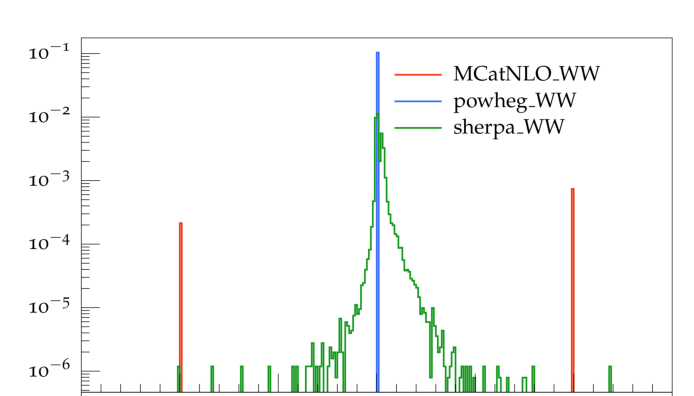
\includegraphics[scale= 0.7]{weight}
\caption{\textit{Distribuzione dei pesi, per differenti generatori Monte Carlo,con  normalizzazione alla sezione d'urto di 1 fb$^{-1}$.}}
\label{weight}
\end{figure}

%Nell'approccio ai Monte Carlo col \textit{parton shower}, si parte dalle sezione d'urto di Born e si aggiungono le correzioni all'ordine successivo dovute al  \textit{parton shower}. Tuttavia nel caso si parta dalla sezione d'urto NLO, sono presenti, aggiungendo il \textit{parton shower}, doppi conteggi degli stessi diagrammi dovuti in particolare all'emissione reale ed al termine negativo proveniente dall'espansione al primo ordine del fattore di forma si Sudakov. 
%Lo scopo di  aM{\footnotesize C@NLO} è di rimuovere questi termini aggiuntivi dall'espressione al NLO. 
%L'eliminazione delle divergenze rende possibile la produzione di due differenti campioni, uno per la parte di Born ($\mathbb{S}$) ed uno per la parte reale ($\mathbb{H}$) ciascuno con un suo proprio peso. $\mathbb{S}$ e $\mathbb{H}$ devono essere accettati in modo proporzionale al loro peso prima di applicare il  \textit{parton shower}.  In generale non si ha la garanzia che i pesi siano positivi (Fig. \ref{weight}), infatti in alcune configurazioni è necessario sottrarre (o in altre aggiungere) eventi.

\paragraph{P{\footnotesize OWHEG}} L'idea alla  base di   P{\footnotesize OWHEG} \cite{Oleari:2010nx} è generare per prima cosa la radiazione più dura, e successivamente  passare l'evento al generatore del \textit{parton shower}. Nei generatori di \textit{parton shower} la produzione, ordinata in impulso trasverso, della radiazione più dura è sempre la prima; quindi  P{\footnotesize OWHEG} sostituisce semplicemente questa con l'emissione al NLO. 
In   P{\footnotesize OWHEG} gli eventi sono prodotti con un peso positivo e costante (Fig. \ref{weight}).


\paragraph{P{\footnotesize YTHIA}8 }  P{\footnotesize YTHIA}8 \cite{bib:pythia} è un generatore che può calcolare il ME per processi con due particelle o partoni nello stato finale, ma soprattutto genera il \textit{parton shower} e la successiva adronizzazione. Il \textit{parton shower} è ordinato in impulso trasverso, $p_T$, e la prima emissione è corretta con il metodo del ripesamento. Per l’adronizzazione utilizza il modello di Lund.  


\paragraph{S{\footnotesize HERPA}}  S{\footnotesize HERPA}  \cite{bib:sherpa} è un generatore Monte Carlo che come PYTHIA8  fornisce una descrizione completa della collisioni adroniche, dal calcolo dell’elemento di matrice, fino all’adronizzazione.  Il \textit{parton shower} include sia le emissioni QCD che quelle dovute alla QED, ovvero i fotoni. Può calcolare il ME per i processi principali (p.e. $gg \rightarrow H$) al NLO e combinare il ME con il  PS. Il codice è scritto completamente in linguaggio C$++$.  

